\documentclass[border=10pt]{standalone} 
\usepackage{tikz, xcolor}
\usepackage{verbatim}

\usetikzlibrary{
matrix,
calc, trees, positioning,
arrows, chains, shapes,
shapes.geometric,
shapes.symbols,
decorations.pathreplacing,
decorations.pathmorphing}

\begin{document}

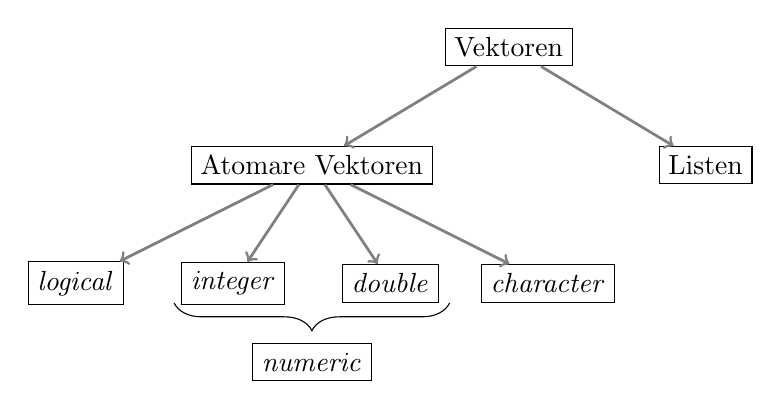
\begin{tikzpicture}[node distance=.8cm, start chain=going below,]

\node[rectangle, text centered, draw=black]
(vectors) at (1.5, 0.5) 
{Vektoren};

\node[rectangle, text centered, draw=black]
(lists) at (4, -1) 
{Listen};

\node[rectangle, text centered, draw=black]
(atom-vectors) at (-1, -1) 
{Atomare Vektoren};

\node[rectangle, text centered, draw=black]
(logical) at (-4, -2.5) 
{\textit{logical}};

\node[rectangle, text centered, draw=black]
(integer) at (-2, -2.5) 
{\textit{integer}};

\node[rectangle, text centered, draw=black]
(double) at (0, -2.5) 
{\textit{double}};

\node[rectangle, text centered, draw=black]
(character) at (2, -2.5) 
{\textit{character}};

\draw[->, line width=1pt, color=gray] (vectors) -- (lists);
\draw[->, line width=1pt, color=gray] (vectors) -- (atom-vectors);
\draw[->, line width=1pt, color=gray] (atom-vectors) -- (logical);
\draw[->, line width=1pt, color=gray] (atom-vectors) -- (integer);
\draw[->, line width=1pt, color=gray] (atom-vectors) -- (double);
\draw[->, line width=1pt, color=gray] (atom-vectors) -- (character);

\draw [decorate,
decoration={brace,
amplitude=10pt},
xshift=-1cm,
yshift=-5cm]
(1.75, 2.25) -- (-1.75, 2.25) node [black,draw, midway, yshift=-0.75cm] 
{\textit{numeric}};

\end{tikzpicture}

\end{document}



